\documentclass{article}
\usepackage{tabularx}
\usepackage{graphicx}
\usepackage{dirtytalk}
\usepackage{pgfplotstable} 
\usepackage{pgfplots}
\usepackage{datatool}
\usepackage{siunitx}
\usepackage[hyphens]{url}
\usepackage{hyperref}
\usepackage{graphicx}
\usepackage{microtype}
\usepackage{float}
\usepackage[style=ieee]{biblatex}
\usepackage{listings}
\usepackage{xcolor}
\usepackage[normalem]{ulem}
\usepackage{dirtytalk}

\definecolor{mygreen}{rgb}{0,0.6,0}
\definecolor{mygray}{rgb}{0.5,0.5,0.5}
\definecolor{mymauve}{rgb}{0.58,0,0.82}

\lstset{
    language=Java,                % Set language to Java
    basicstyle=\ttfamily\footnotesize, % Set font style and size
    keywordstyle=\color{blue},    % Set color for keywords
    stringstyle=\color{mymauve},  % Set color for strings
    commentstyle=\color{mygreen}, % Set color for comments
    numbers=left,                 % Line numbers on the left
    numberstyle=\tiny\color{mygray}, % Style for line numbers
    stepnumber=1,                 % Line number step size
    numbersep=10pt,               % Line number separation
    backgroundcolor=\color{white},% Background color
    showspaces=false,             % Do not show spaces
    showstringspaces=false,       % Do not underline spaces in strings
    showtabs=false,               % Do not show tabs
    frame=single,                 % Draw a frame around the code
    tabsize=4,                    % Set tab size
    captionpos=b,                 % Caption position (bottom)
    breaklines=true,              % Allow line breaking
    breakatwhitespace=false,      % Line breaks only at whitespace
    title=\lstname                % Show the filename of the code
}

\lstdefinestyle{bash}{
    language=bash,                % Set language to Bash
    basicstyle=\ttfamily\footnotesize, % Set font style and size
    keywordstyle=\color{blue},    % Set color for keywords
    stringstyle=\color{mymauve},  % Set color for strings
    commentstyle=\color{mygreen}, % Set color for comments
    numbers=left,                 % Line numbers on the left
    numberstyle=\tiny\color{mygray}, % Style for line numbers
    stepnumber=1,                 % Line number step size
    numbersep=10pt,               % Line number separation
    backgroundcolor=\color{white},% Background color
    showspaces=false,             % Do not show spaces
    showstringspaces=false,       % Do not underline spaces in strings
    showtabs=false,               % Do not show tabs
    frame=single,                 % Draw a frame around the code
    tabsize=4,                    % Set tab size
    captionpos=b,                 % Caption position (bottom)
    breaklines=true,              % Allow line breaking
    breakatwhitespace=false,      % Line breaks only at whitespace
    title=\lstname                % Show the filename of the code
}

\addbibresource{main.bib}

\hypersetup{
    colorlinks=true,
    linkcolor=blue,
    filecolor=blue,      
    urlcolor=blue,
    citecolor=blue,
}

\pgfplotsset{compat=1.18}

\title{\textbf{Lab 1 - Basic Concurrency in Java\\Parallel and Distributed Computing\\DD2443 - Pardis24}}
\author{Names:\\Casper Kristiansson\\Nicole Wijkman\\\\Group 14}
\date{\today}

\begin{document}

\setlength\parindent{0pt}
\setlength{\parskip}{\bigskipamount}

\maketitle

\section{Simple Synchronisation}


\subsection{Race conditions}

\subsubsection{Information}
\textbf{Source files:}

- `task1/MainA.java` (main file)

\textbf{To compile and execute:}
\begin{lstlisting}[style=bash]
javac MainA.java
java MainA
\end{lstlisting}

\subsubsection{Program Explanation}
We began by creating a shared, volatile counter variable that multiple threads could access. Then, we defined a class that implements the \texttt{Runnable} interface, where each thread would increment this counter a million times.

In the \texttt{main} method, we created and started four threads to run the incrementing task simultaneously. After all threads completed their execution, we printed the final value of the counter.

\subsubsection{Discussion}
When running this program we can see that we get the output: \say{\texttt{Counter value: 1091182}}, note that this value differs every time. This is substantially less than the expected value which should be 4,000,000. The reason for this result can be attributed to the nature of both just using the volatile keyword and the fundamentals of how the different threads will read the value of the shared counter. The volatile keyword ensures that each thread can read the latest value of the shared value but its operation is not atomic. This means it will first read the value, increment the value, and then write. Doing this will mean that a lot of the operations will be ignored and increments operations will be lost. As in the title, this is what we call a race condition.


\subsection{Synchronized keyword}
\subsubsection{Information}
\textbf{Source files:}

- `task1/MainB.java` (main file)

\textbf{To compile and execute:}
\begin{lstlisting}[style=bash]
javac MainB.java
java MainB
\end{lstlisting}


\subsubsection{Program Explanation}
We re-used the code from the previous task but modified it by introducing the \texttt{synchronized} keyword to the method responsible for incrementing the shared counter. This ensured that the counter was incremented safely by each thread, preventing the race conditions present in the previous task.

In the \texttt{main} method, we once again created and started four threads to run the incrementing task concurrently. After all threads completed their execution, we measured the execution time and printed the final counter value.

\subsubsection{Discussion}
When running this program we can see that we get the output: \say{\texttt{Counter Value: 4000000
Time: 211451375 ns}}. By using this strategy with the synchronized keyword we can make sure that the result of the shared counter value to always be 4,000,000. Utilizing the synchronized keyword prevents the race condition from overwriting certain increment operations which we saw happening in the previous task.



\subsection{Synchronization performance}
\textbf{Source files:}

- `task1/MainC.java` (main file)

\textbf{To compile and execute:}
\begin{lstlisting}[style=bash]
javac MainC.java
java MainC
\end{lstlisting}


\subsubsection{Program Explanation}
In this task, we measured the performance impact of synchronization across varying numbers of threads. We reused the synchronized increment method from earlier and implemented a \texttt{run\_experiment} method to spawn and join \texttt{n} threads, each incrementing the shared counter.

We chose \texttt{X = 10} warm-up iterations to allow the JVM to optimize and stabilize before measurements begin, and \texttt{Y = 20} measurement iterations to ensure reliable averages while keeping the total runtime of the program manageable. This setup allowed us to observe the performance implications of increasing thread counts from 1 to 64.

To analyze the performance, we calculated the average execution time and standard deviation across multiple runs to assess both consistency and performance overhead. The standard deviation was computed using:


\[
\text{Standard Deviation} = \sqrt{\left(\frac{\sum (\text{time}^2)}{Y}\right) - \left(\text{Average Time}\right)^2}
\]

This allowed us to assess both the consistency and performance overhead introduced by synchronization as the number of threads increased.

We then executed the program on PDC, for the same range of threads, to get a result we could compare with the results of our local machine.


\subsubsection{Result}
As the number of threads increases, we observe a significant rise in execution time. For instance, the average time with 1 thread is about 2.29 milliseconds, but with 64 threads, it reaches over 532 milliseconds. This is due to the overhead of the \texttt{synchronized} keyword, which forces threads to wait their turn to increment the counter.

\begin{table}[H]
\centering
\begin{tabular}{|c|c|c|}
\hline
\textbf{Threads} & \textbf{Average Time (ns)} & \textbf{Standard Deviation (ns)} \\
\hline
1   & 2,227,666.7     & 28,849.36         \\
2   & 21,996,996.05   & 877,982.09        \\
4   & 34,643,375.05   & 2,115,645.74      \\
8   & 69,924,668.7    & 8,190,083.8       \\
16  & 131,321,616.6   & 3,794,384.82      \\
32  & 262,143,381.25  & 15,229,219.75     \\
64  & 508,303,397.9   & 15,938,126.61     \\
\hline
\end{tabular}
\caption{Local Machine (MacBook Pro M1) Results}
\end{table}

\begin{table}[H]
\centering
\begin{tabular}{|c|c|c|}
\hline
\textbf{Threads} & \textbf{Average Time (ns)} & \textbf{Standard Deviation (ns)} \\
\hline
1   & 2,723,026.15    & 148,999.88         \\
2   & 35,170,916.9    & 1,150,519.76       \\
4   & 91,405,393.9    & 12,584,853.82      \\
8   & 244,587,758.45  & 50,243,364.12      \\
16  & 467,120,508.05  & 117,124,377.22     \\
32  & 994,722,323.6   & 146,300,986.62     \\
64  & 2,249,634,642.4 & 329,908,076.21     \\
\hline
\end{tabular}
\caption{PDC Results}
\end{table}

\begin{figure}[H]
    \centering
    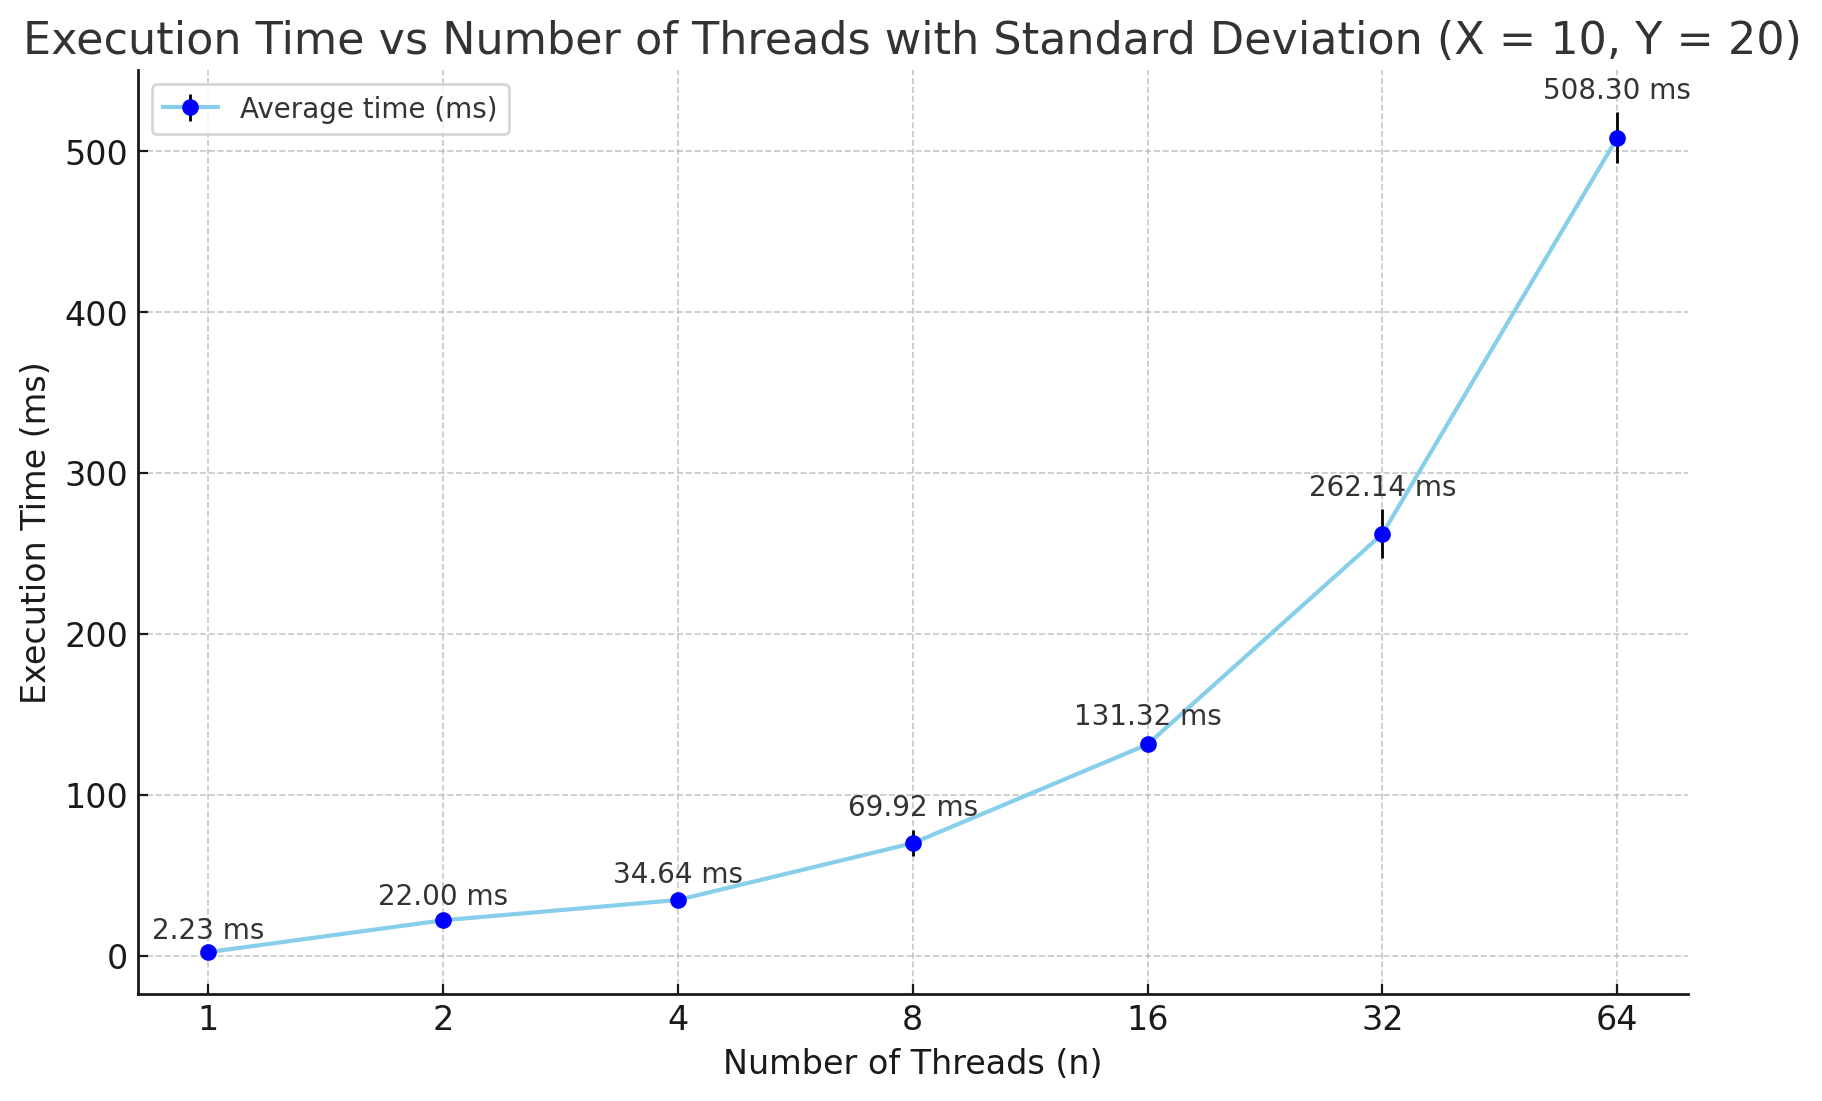
\includegraphics[width=1\linewidth]{LaTex/images/Execution Time vs Number of Threads with Standard Deviation (X = 10, Y = 20).png}
    \caption{Execution Time vs Number of Threads with Standard Deviation}
    \label{fig:1.31}
\end{figure}

\subsubsection{Difference in Performance}

\textbf{Single-Thread Performance:} 
  
  The MacBook Pro M1 is slightly faster with 2,227,666.7 ns compared to the PDC's 2,723,026.15 ns. This is expected as a desktop CPU can often have lower latency for single-threaded operations.

\textbf{Multi-Thread Performance:} 

 As the number of threads increases, the average execution time grows more rapidly on the PDC than on the local MacBook. For example, with 64 threads, the average time on the PDC is approximately 2.25 billion ns, while it is around 508 million ns on the MacBook.
  
  The PDC shows a significantly larger increase in time and standard deviation with more threads, indicating a higher synchronization overhead.

\subsubsection{Discussion}

- \textbf{System Architecture Differences:}
  - \textbf{MacBook Pro M1:} Uses an ARM-based architecture optimized for single-threaded performance and power efficiency. It has a high-performance cache hierarchy and is designed for lower power consumption, contributing to faster single-thread performance and relatively consistent multi-threaded performance up to a certain number of threads.
  - \textbf{PDC (HPE Cray EX):} A high-performance computing system designed for parallel workloads across many CPU cores. The Cray EX system has more complex interconnects and potentially higher overhead for thread synchronization.

- \textbf{Overhead of Synchronization:}
  - \textbf{MacBook Pro M1:} The lower thread count performance suggests lower synchronization overhead.
  - \textbf{PDC (HPE Cray EX):} The increasing overhead, as threads increase, is likely due to the distributed nature of the system.




\newpage
\section{Guarded blocks using wait()/notify()}


\subsection{Asynchronous sender-receiver}

\subsubsection{Information}
\textbf{Source files:}

- `task2/MainA.java` (main file)

\textbf{To compile and execute:}
\begin{lstlisting}[style=bash]
javac MainA.java
java MainA
\end{lstlisting}

\subsubsection{Program Explanation}
In this task, we implemented a simple message-passing scenario using two threads: an \texttt{incrementingThread} and a \texttt{printingThread}. The \texttt{incrementingThread} is responsible for incrementing a shared integer, \texttt{sharedInt}, one million times. The \texttt{printingThread} prints the value of \texttt{sharedInt}.

We deliberately started the \texttt{printingThread} without ensuring that the \\ \texttt{incrementingThread} had finished its task. Since there is no synchronization between the threads, the \texttt{printingThread} may print a value of \texttt{sharedInt} that is neither 0 nor 1,000,000, but some intermediate value. Setting the program up this way demonstrates the lack of synchronization, where the printing operation can occur before the incrementing operation is completed.

\subsubsection{Discussion}
When running this program we can see that we get some different outputs of the final value of \texttt{sharedInt} such as: \texttt{7474}, \texttt{4252}, and \texttt{3204}. The reason for this variation is that the \texttt{printingThread} reads and prints the value of \texttt{sharedInt} without ensuring that the \texttt{incrementingThread} has completed its task. Since there is no synchronization between the threads, the \texttt{printingThread} may print an intermediate value of \texttt{sharedInt} before the incrementing process finishes. This behavior is a direct result of the race condition between the threads, leading to inconsistent and unpredictable results.



\subsection{Busy-waiting receiver} \label{BusyWait}

\subsubsection{Information}
\textbf{Source files:}

- `task2/MainB.java` (main file)

\textbf{To compile and execute:}
\begin{lstlisting}[style=bash]
javac MainB.java
java MainB
\end{lstlisting}

\subsubsection{Program Explanation}
In this task, we modified the program from the previous task to implement a busy-waiting mechanism. We introduced a new shared boolean variable, \texttt{done}, which is declared as \texttt{volatile} and initialized to \texttt{false}. The \texttt{incrementingThread} increments \texttt{sharedInt} one million times and then sets \texttt{done} to \texttt{true} once it has completed its task.

The \texttt{volatile} keyword ensures that changes to \texttt{done} are immediately visible to all threads, preventing the \texttt{printingThread} from getting stuck in an infinite loop due to cached values. The \texttt{printingThread} continuously checks the value of \texttt{done} in a while-loop, busy-waiting until \texttt{done} becomes \texttt{true}. Once \texttt{done} is true, the \texttt{printingThread} prints the final value of \texttt{sharedInt}. This approach ensures that the final value is only printed after the incrementing is finished, eliminating the race condition observed in the previous version.

\subsubsection{Discussion}
When running this program we can see that we consistently get the output: \say{\textit{Final value of sharedInt: 1000000}}. What this indicates is that the busy-waiting mechanism, combined with the \texttt{volatile} keyword for the \texttt{done} variable, effectively ensures that the \texttt{printingThread} waits for the \texttt{incrementingThread} to complete its task before printing the value of \texttt{sharedInt}. The \texttt{volatile} keyword prevents the \texttt{done} variable from being cached, ensuring that the loop in \texttt{printingThread} accurately detects when \texttt{done} becomes \texttt{true}. As a result, the final value of \texttt{sharedInt} is always the expected 1,000,000, demonstrating that this method successfully eliminates the race condition that was present in the previous task.


\subsection{Waiting with guarded block} \label{GuardBlock}

\subsubsection{Information}
\textbf{Source files:}

- `task2/MainC.java` (main file)

\textbf{To compile and execute:}
\begin{lstlisting}[style=bash]
javac MainC.java
java MainC
\end{lstlisting}

\subsubsection{Program Explanation}
In this task, we modified the previous program further by replacing the busy-waiting mechanism with a guarded block using \texttt{synchronized}, \texttt{wait()}, and \texttt{notify()}. The \texttt{incrementingThread} increments the shared integer \texttt{sharedInt} one million times. Once it completes, it enters a synchronized block to set the \texttt{done} flag to \texttt{true} and calls \texttt{notify()} to signal the \texttt{printingThread} that the incrementing is complete.

The \texttt{printingThread} now uses a synchronized block and a \texttt{while} loop to wait for the notification. It calls \texttt{wait()} and only proceeds to print the final value of \texttt{sharedInt} when it receives the notification from the \texttt{incrementingThread}. This approach replaces the inefficient busy-waiting with a more efficient wait-notify mechanism, ensuring that the \texttt{printingThread} only proceeds after the incrementing is finished, while also handling potential spurious wake-ups by rechecking the condition in the \texttt{while} loop.

\subsubsection{Discussion}
When running the program for this task we can see that we consistently get the output: \say{\textit{Final value of sharedInt: 1000000}}. This result indicates that using the \texttt{synchronized}, \texttt{wait()}, and \texttt{notify()} mechanism effectively coordinates the execution of the \texttt{incrementingThread} and \texttt{printingThread}. The \texttt{printingThread} waits correctly for the \texttt{incrementingThread} to complete its task before printing the value of \texttt{sharedInt}. The use of a synchronized block and the \texttt{wait()} method ensures that the \texttt{printingThread} only proceeds after receiving the notification, eliminating any race conditions and avoiding unnecessary CPU usage caused by busy-waiting. As a result, the final value of \texttt{sharedInt} is always the expected 1,000,000, demonstrating that this approach is both efficient and reliable.



\subsection{Guarded block on performance}

\subsubsection{Information}
\textbf{Source files:}

- `task2/MainD.java` (main file)

\textbf{To compile and execute:}
\begin{lstlisting}[style=bash]
javac MainD.java
java MainD
\end{lstlisting}

\subsubsection{Program Explanation}
In this task, we compared the performance of a busy-waiting approach against a guarded block approach by modifying the programs from Section \ref{BusyWait} and Section \ref{GuardBlock}. We measured the delay between the completion of the \texttt{incrementingThread} and the \texttt{printingThread} receiving the notification, using \texttt{System.nanoTime()}.

We implemented two methods: \texttt{runExperimentsBusyWaiting()} and \\ \texttt{runExperimentsGuardedBlock()}. The former method employs a busy-waiting mechanism where the \texttt{printingThread} continually checks the \texttt{done} flag until the \texttt{incrementingThread} completes. The latter uses a guarded block, where the \texttt{printingThread} waits for a notification from the \texttt{incrementingThread} before proceeding.

To assess the performance, we ran both methods locally, with a warm-up phase followed by multiple measurement iterations. We recorded and compared the delays for both approaches to analyze the impact of guarded blocks on performance.

\subsubsection{Discussion}
From what we can see after running a test both comparing the average time of running up to 1000 tests is that the difference is really small but most of the time the guarded block has better performance. We generally saw around a 5-10\% faster execution time. Using a guarded block is extremely better in terms of the performance of the CPU because we are not constantly checking a flag as in part B. Checking a busy flag in a while loop over and over is extremely CPU heavy which then can affect the actual counting process. However, we did see some outlier tests where the guarded block approach took 5-10\% longer to execute.




\newpage
\section{Producer-Consumer Buffer using Condition Variables}

\subsection{Producer-consumer buffer and Buffer class}

\subsubsection{Information}
\textbf{Source files:}

- `task3/Main.java` (main file)

\textbf{To compile and execute:}
\begin{lstlisting}[style=bash]
javac Main.java
java Main
\end{lstlisting}

\subsubsection{Program Explanation}
In this task, we implemented a producer-consumer buffer using Java's \\ \texttt{ReentrantLock} and \texttt{Condition} variables. The \texttt{Buffer} class manages a queue with a fixed capacity \(N\) and ensures thread-safe interactions between producer and consumer threads.

The \texttt{Buffer} class includes three primary methods:
\begin{itemize}
    \item \texttt{add(int i)}: Allows the producer to insert integers into the buffer. If the buffer is full, the producer waits until space is available.
    \item \texttt{remove()}: Allows the consumer to remove and return integers from the buffer. If the buffer is empty, the consumer waits until an item is available.
    \item \texttt{close()}: Closes the buffer, preventing any further additions but allowing remaining items to be consumed.
\end{itemize}

The \texttt{Producer} thread adds 1,000,000 integers to the buffer, then closes it. The \texttt{Consumer} thread continuously removes integers from the buffer and prints them. All of the synchronization is handled within the \texttt{Buffer} class, which ensures safe interaction between the producer and consumer without direct synchronization in their respective code.


\subsubsection{Discussion}
In short, the program segments the generation of numbers between \texttt{x} and \texttt{x + buffer size}. A consumer then consumes these numbers. If the buffer becomes full, the producer will wait until space becomes available. If the buffer becomes empty, the consumer will wait until new items are added. Both the producer and consumer wake up using the \texttt{ReentrantLock} and \texttt{Condition} classes, which handle the synchronization efficiently.



\newpage
\section{Counting Semaphore}

\subsection{Basic Semaphore Counting and Testing Semaphore with Various Counter Values and Thread Counts}

\subsubsection{Information}
\textbf{Source files:}

- `task4/Main.java` (main file)

\textbf{To compile and execute:}
\begin{lstlisting}[style=bash]
javac Main.java
java Main
\end{lstlisting}

\subsubsection{Program Explanation}
In this task, we implemented a counting semaphore using Java's \texttt{synchronized}, \texttt{wait()}, and \texttt{notify()} mechanisms. The \texttt{CountingSemaphore} class manages a counter that controls access to a shared resource. The semaphore supports two primary operations: \texttt{s\_wait()} and \texttt{signal()}.

\begin{itemize}
    \item \texttt{s\_wait()}: Decrements the semaphore counter. If the counter is negative, the thread waits until a resource becomes available.
    \item \texttt{signal()}: Increments the semaphore counter. If the counter is non-positive, it notifies a waiting thread that a resource is now available.
\end{itemize}

We tested the semaphore with a \texttt{Runner} class, where multiple threads attempt to acquire the semaphore, perform a task we have simulated, and then release the semaphore. The main method initializes the semaphore with a count of 3 and starts with 5 threads to observe the semaphore's behavior under concurrent conditions.

\subsubsection{Discussion}
During this exercise, we identified a potential issue in regard to the exercise instruction: \say{If the value was negative prior to the increment, wake one thread waiting on the semaphore.} The issue with this is that with this structure a deadlock could occur. Specifically, with our current solution, if the count is -1 and a resource releases a semaphore while a thread is still waiting, the waiting thread will be notified. However, when the thread that was sleeping rechecks the condition \texttt{count < 0}, it may go back to sleep and wait again, potentially leading to a situation where no progress is made. If the current count is 0 and we increase it, a thread might still be asleep. This means that running the program multiple times with 3 semaphores and 5 threads will sometimes cause a deadlock. It does, however, not seem to get stuck for other inputs.


\newpage
\section{Dining Philosophers}
\subsection{Model the Dining Philosophers}

\subsubsection{Information}
\textbf{Source files:}

- `task5/MainA.java` (main file)

\textbf{To compile and execute:}
\begin{lstlisting}[style=bash]
javac MainA.java
java MainA
\end{lstlisting}

\subsubsection{Program Explanation}
In this task, we modeled the classic Dining Philosophers problem, where a group of philosophers alternates between thinking and eating. The philosophers sit around a circular table, with one chopstick placed between each pair of adjacent philosophers. To eat, a philosopher must first pick up both chopsticks adjacent to them. However, they can only eat if they have successfully picked up both chopsticks. After eating, they place the chopsticks back on the table and return to thinking.

Our implementation aims to solve this problem using Java’s \texttt{ReentrantLock} to represent each chopstick. Each philosopher is modeled as a thread that alternates between thinking and attempting to eat. To prevent deadlock, philosophers pick up the left chopstick first, then the right chopstick. This approach, however, can still lead to deadlock if all philosophers pick up their left chopstick simultaneously and then wait for the right one.

In our solution, we assign each philosopher two chopsticks—the left and right—by using modular arithmetic to ensure the last philosopher correctly shares chopsticks with the first philosopher. Each philosopher thread runs in an infinite loop, simulating the process of thinking, attempting to acquire the chopsticks, eating, and then releasing the chopsticks. This setup allows us to observe the deadlocks and test different strategies for preventing them.

\subsubsection{Discussion}
When testing with five philosophers, we observed that the program could lead to a deadlock, particularly when each philosopher picks up their left chopstick simultaneously and then waits indefinitely for the right one. This deadlock occurs because all philosophers are holding one chopstick, preventing any from acquiring the second chopstick needed to eat.

As the number of philosophers increases, the likelihood and speed of encountering a deadlock rise due to more threads competing for the limited chopsticks. This emphasizes the need for strategies to prevent deadlock, such as implementing resource acquisition hierarchies or introducing random delays before picking up chopsticks. But we also found that when minimizing both the delay for thinking and eating to 1ms we would sometimes with just 5 philosophers reach a deadlock on the first iteration of the code.

\subsection{Java Debug}

We are using Visual Studio Code to develop our solution, in which we additionally also have the Java extension pack. This allows to debug the code directly in the editor. By pausing the execution when a deadlock occurs, we can inspect the state of each thread to understand the cause of the issue.  For example, by pausing the execution in our code we can see that each thread is parked and is trying to acquire the right chopstick. By pausing we also acquire additional information, such as the current stack trace. This allows us to see the progress of the program and the different values of objects.  For instance, we can identify specific instances of \texttt{ReentrantLock}, labeled as \texttt{ReentrantLock@{id}} (e.g., \texttt{ReentrantLock@39}), which allows us to determine which thread currently holds a particular lock.

In addition to the IDE-based debugging, there is the \texttt{jstack} tool, which is part of the Java Development Kit (JDK). \texttt{jstack} generates a thread dump that shows the current state of threads in a Java process. When a deadlock occurs, \texttt{jstack} can help identify the specific threads involved and the resources they are waiting for. This makes it easier to pinpoint the cause of the deadlock. By analyzing the thread dump, we can see which locks are held and which ones are being waited on. This thus provides a clear view of the deadlock situation.



\subsection{Solution to the Dining Philosophers problem}

\subsubsection{Information}
\textbf{Source files:}

- `task5/MainB.java` (main file)

\textbf{To compile and execute:}
\begin{lstlisting}[style=bash]
javac MainB.java
java MainB
\end{lstlisting}

\subsubsection{Program Explanation}
In this task, we implemented a solution to the Dining Philosophers problem, focusing on ensuring that our solution is both deadlock-free and starvation-free \cite{85Dining71:online}.

To prevent deadlock, we utilized a semaphore to limit the number of philosophers who can attempt to pick up chopsticks simultaneously. More specifically, the semaphore allows \texttt{numberOfPhilosophers - 1} philosophers to access the chopsticks at any given time. What this ensures is that at least one philosopher will always be able to pick up both of the chopsticks to eat, which breaks the potential circular wait condition that could lead to a deadlock.

Our solution also prevents starvation and guarantees fairness by utilizing the semaphore's FIFO (First-in, First-out) queue. This will ensure that each philosopher gets a turn to eat, without being indefinitely blocked by others. The result is that no philosopher will be forced to wait infinitely long, and this ensures that all philosophers eventually get to eat. This makes the solution both deadlock-free and starvation-free.

\subsubsection{Discussion}
The reason why this solution is effective is because of the structure of using semaphores. By allowing \texttt{n-1} semaphores to be acquired there will always be at least one that can eat with both chopsticks essential to dealing with the issue that all left chopsticks will be picked up. Secondly, the semaphore allows for fairness because it follows the FIFO queue system which means that no thread will end up starving.


\newpage
\printbibliography

\end{document}